\section{Problem Statement}
\label{sec:problem_statement}

In this section, we discuss the details of a robot wingman in a human-robot team and define a model for the wingman path planning problem in a human-robot team search task.

We consider the search problem on a discrete map.
Let $ I $ denote the set of cells in the map.
We refer to the object or person of interest as the \emph{search target}.
For the cordon and search problem, we are using an occupancy grid representation where for each cell in the discretized space we classify the cell as being either occupied by a search target.
For each cell $ i \in I $, let $ S_{i} $ denote the binary random variable that whether there is a search target in cell $ i $.
$ P(S_{i}) $ is its probability and $ H(S_{i}) $ is its entropy.

We define a flank support range $ \gamma_{flank} $ to model the robot wingman constraint. 
This range determines the area that a robot wingman is expected to stay in when a human is moving, which is shown in Figure \ref{fig:Wingman}.
Let $ x_{t} $ denote the position of the robot wingman at time $ t $ and $ y^{h}_{t} $ denote the position of the human at time $ t $.
The robot wingman constraint requires that $ \forall t, || x_{t} - y^{h}_{t} || \leq \gamma_{flank} $.
For a discretized state space, this same definition holds as long as we define the human's and the robot's positions as the center of the cell.
In a search task, we assume that both human and robot can observe a circular area around themselves, which is defined in the same way as the flank support range as shown in Figure \ref{fig:Wingman}.
The observation ranges are $ \gamma^{human}_{obsRange} $ and $ \gamma^{robot}_{obsRange} $.
This means that an agent can observe not only the visited cell but neighboring cells in a range.
We use a neighbor function $ N^{a}_{r}(\cdot) $ to denote a set of cells satisfying some constraints of a given node, in which $ a $ denotes the application usage and $ r $ gives the range parameter.
$ N^{flank}(\cdot) $ defines the allowable cells for the robot's location given the human's position, $ N^{human}_{obsRange}(\cdot) $ and $ N^{robot}_{obsRange}(\cdot) $ define the observable cells given a position of a human and a robot, respectively.

The discrete map can be used to form the topology defining the connections between accessible positions.
Figure \ref{fig:LayerStructure} illustrates how the topological graph is formed from a real world map.
In this paper, we consider path planning on a topological graph, in which there is dependence on a human path.

\begin{figure}[htbp]
\centering
\includegraphics[width=0.45\textwidth]{./images/LayerStructure.pdf}
\caption{A layer structure of problem abstraction from real world of search space to topological description.}
\label{fig:LayerStructure}
\end{figure}

\subsection{Human Path Dependence}
\label{subsec:human_path_dependence}
 
A path of an agent is expressed as a sequence of vertices in a topology. 
In a time length of $ T $, let a vector $ Y^{h} = [y^{h}_{1}, y^{h}_{2} , \cdots , y^{h}_{T}] $ define a path of the human.
Similarly, we have a path of the robot as $ X = [x_{1}, x_{2} , \cdots , x_{T}] $.
Note that this assumes that the robot's speed matches the human's speed.
$ N^{human}_{obsRange}( y^{h}_{t} ) $ determines a set of observations made by the human at location $ y^{h}_{t} $, which is denoted as  $ O^{Y^{h}}_{t} $.
Let $ \mathbf{O}^{Y^{h}} = \{ O^{Y^{h}}_{1}, \cdots , O^{Y^{h}}_{T-1}, O^{Y^{h}}_{T} \} $ denote the sequence of these sets.
Define $ \mathbf{O}^{X} $ similarly.

We adopt Bayes rule to update the probability estimation through observations, which results in entropy reduction.
By considering the entropy reduction as information gathered by the robot, our goal is to maximize the information gained by moving the robot in the world.
In this paper, we focus on an offline path planning problem under four assumptions \ref{Assumption1} , \ref{Assumption2} , \ref{Assumption3} and \ref{Assumption4}.

\begin{Hyp}
\label{Assumption1}
The human path is known.
\end{Hyp}

\begin{Hyp}
\label{Assumption2}
There is a human observation model, which can be used to predict what the human will and will not see in the world.
\end{Hyp}

\begin{Hyp}
\label{Assumption3}
The search environment is time-invariant.
\end{Hyp}

\begin{Hyp}
\label{Assumption4}
The observation models of both the human and the robot are time-invariant and spatially independent.
\end{Hyp}

Assumptions \ref{Assumption1} and \ref{Assumption2} allow us to determine the distribution of $ \mathbf{O}^{Y^{h}} $, which is applied to update the estimated probability on where the search target is before doing path planning of the robot.
By Assumptions \ref{Assumption3} and \ref{Assumption4}, we can derive Property \ref{prop:orderIndependence}.

\begin{propty}
\label{prop:orderIndependence}
Given a path $ X = [ x_{1}, x_{2} , \cdots , x_{t} ]^{T} $, the total information can be collected is independent with the visiting sequence.
\begin{proof}
See the proof in Appendix \ref{app:order_independence}
\end{proof}
\end{propty}


We use conditional mutual information to evaluate the information gain of the robot.
In equation \eqref{eq:condMutInf}, this means that the entropy reduction on uncertainty estimation on the search space $ \mathbf{S} $ due to the observation of a robot $ \mathbf{O}^{X} $ when the observation of a human $ \mathbf{O}^{Y^{h}} $ is given.

\begin{equation}
\label{eq:condMutInf}
\begin{aligned}
I(\mathbf{S}; \mathbf{O}^{X} \mid \mathbf{O}^{Y^{h}}) & = H(\mathbf{S} \mid \mathbf{O}^{Y^{h}}) - H(\mathbf{S} \mid \mathbf{O}^{X},\mathbf{O}^{Y^{h}})\\
& = H(\mathbf{O}^{X} \mid \mathbf{O}^{Y^{h}}) - H(\mathbf{O}^{X} \mid \mathbf{O}^{Y^{h}}, \mathbf{S}).
\end{aligned}
\end{equation}

The information maximization of a robot in a search problem can be defined as an optimization problem, which is:

\begin{equation}
\label{eq:objFunc}
\begin{aligned}
Objective: X^{*} = \underset{X}{\arg\max} [I(\mathbf{S}; \mathbf{O}^{X} \mid \mathbf{O}^{Y^{h}})] \\
Constraint: \forall t, x^{t} \in N^{flank}(y_{t}) \cap N^{robot}_{1}(x^{t-1}) 
\end{aligned}
\end{equation}

Due to the existence of the potential overlap between robot observation regions of different times, the entropy reduction by $ O^{X}_{t} $ depends on $ O^{X}_{1} , \cdots , O^{X}_{t-1} $ as well.
This is stated in Lemma \ref{Lemma1}.

\begin{lem} 
\label{Lemma1}
When the human observation $ \mathbf{O}^{Y} $ is known, we can factor the objective in equation \eqref{eq:condMutInf} into a chain rule form,
\begin{equation}
\label{eq:offHmPathChain}
\begin{aligned}
I(\mathbf{S}; \mathbf{O}^{X} \mid \mathbf{O}^{Y^{h}}) & = \sum_{t=1}^{T} H(O_{t}^{X} \mid O_{1}^{X} , \cdots , O_{t-1}^{X}, \mathbf{O}^{Y^{h}}) - \sum_{t=1}^{T} H(O_{t}^{X} \mid O_{1}^{X} , \cdots , O_{t-1}^{X}, \mathbf{S}, \mathbf{O}^{Y^{h}}) \\
& = \sum_{t=1}^{T} I(O^{X}_{t} ; \mathbf{S} \mid O^{X}_{1} , \cdots , O^{X}_{t-1}, \mathbf{O}^{Y^{h}})
\end{aligned}
\end{equation}
\begin{proof}
The proof follows trivially from the definition of conditional probability and conditional mutual information. 
The detail is given in Appendix.
\end{proof}
\end{lem}

In equation \eqref{eq:offHmPathChain}, we can express the maximum total information as a summation of maximizing information at each step, which indicates a sequential substructure in solving the maximization problem.
Thus we look into the solution space and the optimization at each single planning step.

\subsection{Unfold Solution Space of Single Step Through Time}
\label{subsec:unfold_solution_space}

%We find that there exists a temporal-space relationship between a robot wingman and a human.
%a solution space at one time step for a robot is a set of positions defined by $ N^{flank}() $ and a human position $ y^{h}_{t} $.
When assumption \ref{Assumption1} stands, the solution space of a robot wingman at a single time step is determined by $ N^{flank}() $ and a human position $ y^{h}_{t} $. Unfolding the solution spaces at different time steps generates a multi-partite graph for path planning. Figure \ref{fig:MultiPartite} gives an example. A partition of time $ t $ indicates a set of vertices which are allowed for the robot wingman to visit at time $ t $. As expressed in Figure  \ref{fig:LayerStructure}, the topological graph determines the edges between vertices in the multi-partite graph.

\begin{mydef}[\textbf{Multi-Partite Graph}]
\label{def:multi_partite}
The multi-partite graph $ G = (V, E, T) $ is defined as
\begin{itemize}
\item The number of partitions is $ T $.
\item The vertex set $ V $ is defined as $ V = \cup_{t=1}^{T} V(t) $.
Each partition $ V(t) $ is a set of vertices $ v^{i}_{t} $, where $ t $ indicates which partition the vertex $ x $ is in and $ i $ indicates the index of this vertex.
\item Edges are directed, originating from vertices in set $ V(t) $ to vertices in set $ V(t+1) $.
Let $ v^{i}_{t} \in V(t) $ and $ v^{j}_{t+1} \in V(t+1) $.
A directed edge $ (v^{i}_{t}, v^{j}_{t+1}) $ connects vertices $ v^{i}_{t} $ and $ v^{j}_{t+1} $. 
\end{itemize}
\end{mydef}

Figure \ref{fig:MultiPartite} gives an example on a multi-partite graph converted from a topological graph.
Each partition $ V(t) $ is determined by $ V(t) = N^{flank} ( y^{h}_{t} ) $.
There is a directed edge that connects vertices $ v^{i}_{t} $ and $ v^{j}_{t+1} $ only if there is an edge that connects them in the topological graph.

\begin{figure}[htbp]
\centering
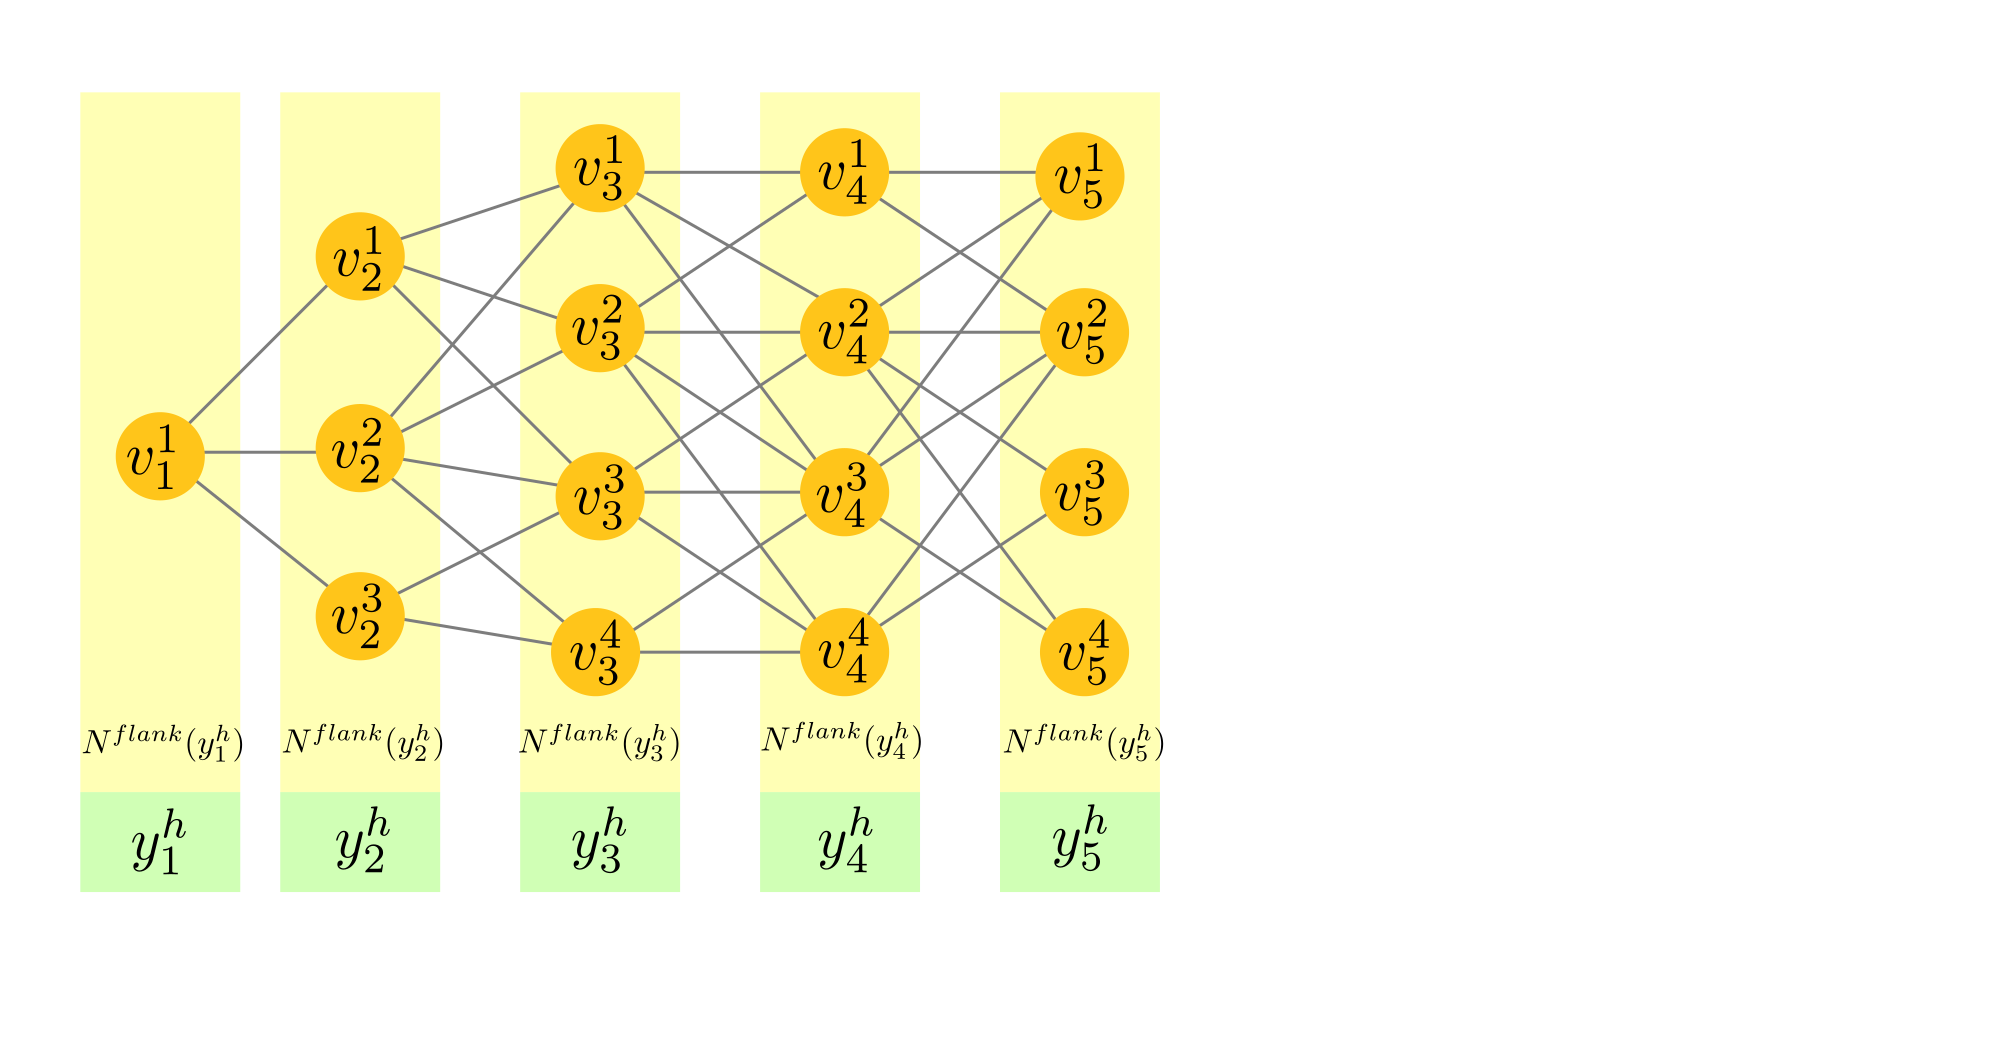
\includegraphics[width=0.4\textwidth]{./images/MultiPartite.pdf}
\caption{A multi-partite graph for robot wingman search.}
\label{fig:MultiPartite}
\end{figure}
 
If a vertex $ v^{i}_{t} $ cannot be reached from any vertex in partition $ V(t-1) $ or does not go into any vertex in partition $ V(t+1) $, it will never be in a path of length $ T $.
Here we use a pruning process to remove those ``useless'' vertices in a planning problem.
The pruning process consists of forward pruning and backward pruning.
The forward pruning starts from partition $ V(2) $ to partition $ V(T) $.
Any vertex that has no in edge and its incident edges will be removed.
The backward pruning starts from partition $ V(T-1) $ to partition $ V(1) $.
Any vertex that has no out edge and its incident edges will be removed.
\footnote{In forward pruning, removing a vertex and its incident edges in $ V(t) $ might only make vertices in $ V(t+1) $ having no in edge.
Those vertices will be removed when pruning in $ V(t+1) $.
Similarly, in backward pruning, removing a vertex and its incident edges in $ V(t) $ might only make vertices in $ V(t-1) $ having no out edge.
Those vertices will be removed when pruning in $ V(t-1) $.  
This means that two prunings will not make any vertex has no in edge or has no out edge.
Thus, the properties of ``non-terminating'' and ``reachable'' can be guaranteed.}
After the pruning, the multi-partite graph has below two properties.
\begin{itemize}
\item \emph{Non-terminating:} From $ V(1) $ to $ V(T-1) $, any vertex has an out edge to a vertex in the next partition, which ensures that $ \forall t \in \{ 1 , \cdots , T-1 \} \forall v^{i}_{ t } \in V( t )  ( deg^{+}(v^{i}_{ t }) > 0 )  $.
\item \emph{Reachable:} From $ V(T) $ to $ V(2) $, any vertex has an in edge from a vertex in the previous partition, which ensures that $ \forall t \in \{ 2, \cdots , T \} \forall v^{i}_{ t } \in V( t )  ( deg^{-}(v^{i}_{ t }) > 0 )  $. 
\end{itemize}